\documentclass[../main.tex]{subfiles}
\begin{document}
\section{导航规划融合优化}
\subsection{传统导航规划存在的问题}
\begin{itemize}
    \item 在路径规划中不考虑机器人的\textbf{运动学约束},导致轨迹规划不能跟踪实现所有路径\footnote{对A*算法而言,随机生成的路径规划点对中大概只有8.3\%可以被正常执行}
    \item 如果实时避障偏离路径,避障规划和轨迹控制器\textbf{没有}如何到达目标的\textbf{全局信息}
\end{itemize}
\subsection{导航规划优化方法}
\begin{enumerate}
    \item \textbf{混合A*}
        \begin{itemize}
            \begin{figure}[H]
                \centering
                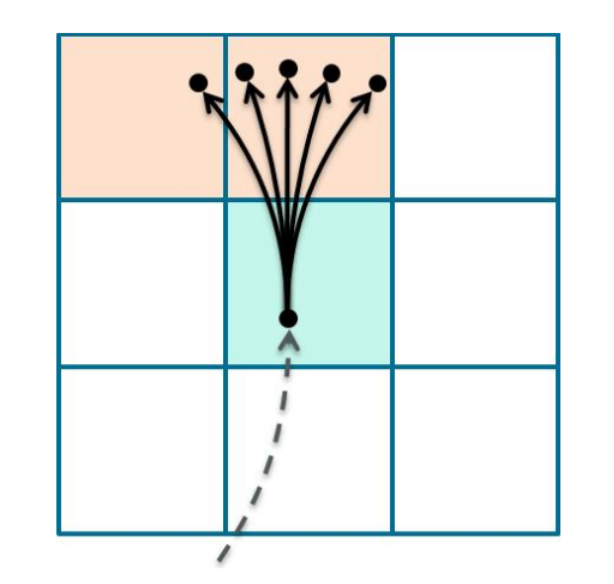
\includegraphics[width=0.3\textwidth]{images/yundongjiyuan.png}
                \caption{运动基元示意图}
            \end{figure}
            \item \textbf{运动基元}:指机器人\textbf{一个时间片}内能够实现的\textbf{平移和旋转}运动,受机器人的最大加速度和最大速度的约束,同时要求满足以下条件:
                \begin{enumerate}
                    \item 路径距离要足够离开当前网格
                    \item 路径曲率受最大转向角约束
                    \item 朝向变化是离散转角步长的倍数
                \end{enumerate}
            \item \textbf{针对问题}:传统A*得到的是直线段组成的路径;混合A*得到的\textbf{路径等同于轨迹},确保了机器人运动的平滑性和可实现性
            \begin{figure}[H]
                \centering
                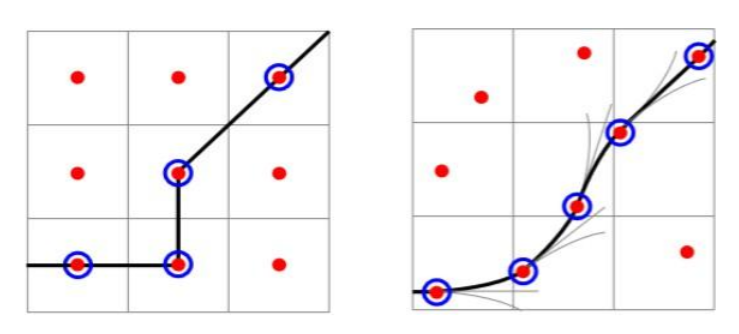
\includegraphics[width=0.5\textwidth]{images/mixedAs.png}
                \caption{传统A*与混合A*的路径对比}
            \end{figure}

            \begin{table}[H]
              \centering
              \caption{A* 与 混合A* 的对比}
              \begin{tabular}{@{}l
                  >{\raggedright\arraybackslash}p{4cm}
                  >{\raggedright\arraybackslash}p{6cm}@{}}
                \toprule
                 & \textbf{A*} & \textbf{混合A*} \\
                \midrule
                \textbf{机器人状态表示} & 位置$(x, y)$ & 位姿$(x, y, \theta)$ \\
                                       & 离散 & 连续 \\
                \midrule
                \textbf{扩张搜索策略} &
                  相邻节点,每个相邻栅格是一个搜索节点 &
                  预定义运动基元,同一栅格可存在多个搜索节点 \\
                \bottomrule
              \end{tabular}
            \end{table}


        \end{itemize}
    \item \textbf{弹性带算法(ELASTIC BAND)}
        \begin{itemize}
            \item \textbf{基本思想}:根据环境感知对所规划路径进行实时变形,同时实现局部避障和路径平滑\footnote{在执行局部避障的同时维护着一条完整的到达目标点的无碰路径}
            \item \textbf{基本原理}:对路径上的点施加两种力:
                \begin{itemize}
                    \item \textbf{内部收缩力}:用于模拟拉伸弹性带中的张力并消除路径中的松弛
                    \item \textbf{外部排斥力}:用于模拟障碍物排斥,抵消张力并拉开机器人与障碍物之间的距离
                \end{itemize}
                进而有:
                \begin{itemize}
                    \item 两种力使弹性带变形直至达到平衡
                    \item 动态障碍物会改变力重新达成平衡
                \end{itemize}
                    \begin{figure}[H]
                        \centering
                        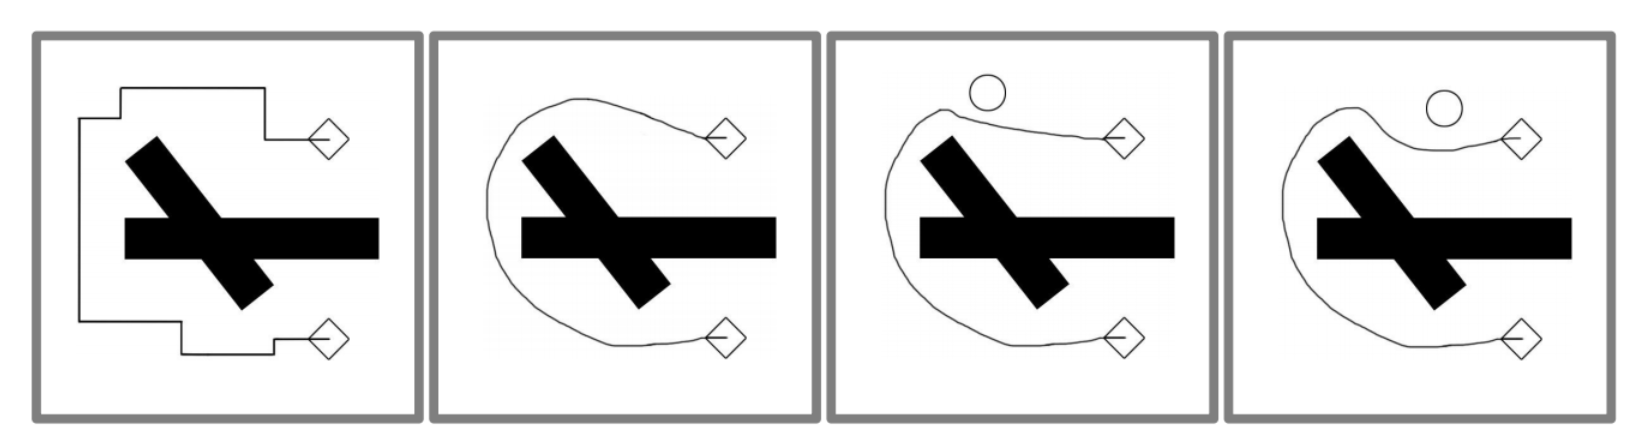
\includegraphics[width=0.7\textwidth]{images/tanxingdai.png}
                        \caption{弹性带算法效果示意图}
                    \end{figure}
            \item \textbf{面临问题}:
                \begin{itemize}
                    \item \textbf{离散→连续}路径为一系列离散点表示,弹性带算法必须根据这些点生成一条连续的曲线
                    \item \textbf{无碰检测}:所生成的连续曲线必须是安全无碰的,而曲线无碰检测是一件耗时的工作。
                \end{itemize}
                    \begin{figure}[H]
                        \centering
                        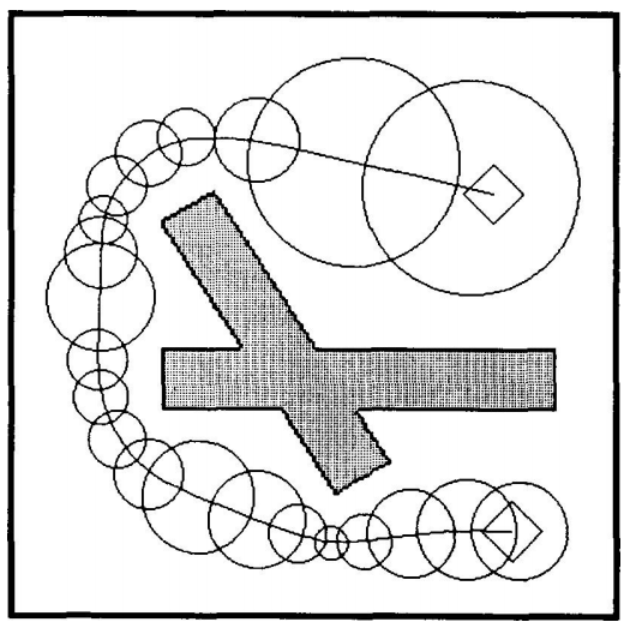
\includegraphics[width=0.2\textwidth]{images/BUBBLE.png}
                        \caption{弹性带算法+气泡示意图}
                    \end{figure}
            \item \textbf{解决方案}:\textbf{气泡BUBBLE}:采用\textbf{气泡集合}来\textbf{近似}表示规划路径附近的自由空间,而不是计算表达整个自由空间\\
                \small\kaishu{
                \begin{itemize}
                    \item 每一个气泡是自由空间的一个子集,以路径点为中心,以该路径点与最近障碍物之间的安全距离为半径
                    \item 路径表示为一系列路径点和由路径点长成的气泡,只要相邻气泡有一定的相互覆盖,就能确保该路径是安全的
                \end{itemize}}
                具体计算过程如下:
                \begin{enumerate}
    
    \item \textcolor{red}{生成用气泡表示的路径}\\\textbf{气泡的数学描述}
    在姿态空间中,设气泡在点 $\mathbf{b}$ 处,其定义为:
    \[
        B(\mathbf{b}) = \{ \mathbf{q} \mid \| \mathbf{b} - \mathbf{q} \|_2 < \rho(\mathbf{b}) \}
    \]
    其中,$\rho(\mathbf{b})$ 表示机器人在点 $\mathbf{b}$ 处与环境中障碍物之间的最小安全距离函数。  

    若考虑机器人姿态旋转因素,则气泡可定义为:
    \[
        B(\mathbf{b}) = \{ \mathbf{q} : D(\mathbf{b} - \mathbf{q}) < \rho(\mathbf{b}) \}
    \]
    其中距离函数 $D(\Delta \mathbf{b})$ 为:
    \[
        D(\Delta \mathbf{b}) = \sqrt{(\Delta b_x)^2 + (\Delta b_y)^2} + r \left| \Delta b_\theta \right|_{\max}
    \]
    其中 $r$ 表示旋转半径\footnote{可用复杂模型表示气泡,需要在计算效率和表示个数上进行折中考虑}。


    \item     \textcolor{red}{基于相邻气泡点有收缩力、障碍物有推斥力的思想,依次来回扫描并移动各个气泡,根据虚拟力计算每个气泡的移动距离和方向}\\\textbf{虚拟力计算}:
    \vspace{1em}
    虚拟力由收缩力(吸引力)与推斥力两部分构成。

    \begin{itemize}
        \item \textbf{收缩力 / 吸引力:}
        \[
            \mathbf{f}_c = k_c \left( 
            \frac{\mathbf{b}_{i-1} - \mathbf{b}_i}{\|\mathbf{b}_{i-1} - \mathbf{b}_i\|_2} + 
            \frac{\mathbf{b}_{i+1} - \mathbf{b}_i}{\|\mathbf{b}_{i+1} - \mathbf{b}_i\|_2} 
            \right)
        \]
        其中,$k_c$ 为全局收缩系数。

        \item \textbf{推斥力:} 沿着气泡尺寸变化最大方向施加:
        \[
            \mathbf{f}_r =
            \begin{cases}
                k_r (\rho_0 - \rho)\dfrac{\partial \rho}{\partial \mathbf{b}}, & \rho < \rho_0 \\
                0, & \rho \geq \rho_0
            \end{cases}
        \]
        其中,$k_r$ 为全局推斥系数,$\rho_0$ 为力作用距离阈值。

        梯度项可数值近似为:
        \[
            \dfrac{\partial \rho}{\partial \mathbf{b}} = 
            \dfrac{1}{2h} 
            \left[
            \rho(\mathbf{b} - h\mathbf{x}) - \rho(\mathbf{b} + h\mathbf{x}),\;
            \rho(\mathbf{b} - h\mathbf{y}) - \rho(\mathbf{b} + h\mathbf{y})
            \right]
        \]
        其中 $h$ 为步长。\\
    \item 根据合力调整位置,气泡沿着力的方向移动:
    \[
        \mathbf{b}_{\text{new}} = \mathbf{b}_{\text{old}} + \alpha \mathbf{f}_{\text{total}}
    \]
    其中,$\alpha$ 为比例系数,可取 $\alpha = \rho(\mathbf{b}_{\text{old}})$,表示移动距离与原气泡尺寸成比例。

    该更新方程通过下坡梯度搜索方式寻找弹性带平衡点,收敛较慢时可采用增加惯性项或二阶控制系统以加快收敛。
    \end{itemize}
    
    \item \textcolor{red}{为了确保弹性带构成的路径安全无碰,要求每个气泡与它两边的相邻气泡有重叠区域,需根据需要增加新气泡或删除多余气泡}\\\textbf{气泡的插入与删除}:
    \begin{itemize}
        \item \textbf{增加新气泡:} 若新位置气泡与相邻气泡未重叠,则弹性带会断裂,需要在现有气泡间插入新气泡以重新连接路径。
        \item \textbf{删除多余气泡:} 为降低计算复杂度,可扫描气泡序列,检查相邻气泡是否重叠,若可在不破坏弹性带的情况下移除,则删除冗余气泡。
        \item \textbf{震荡修正:} 针对新气泡插入或多余气泡删除造成的路径震荡问题,修正虚拟力计算,去除切向分量:
        \[
            \mathbf{f}^* = \mathbf{f} -
            \mathbf{f} \dfrac{(\mathbf{b}_{i-1} - \mathbf{b}_{i+1})(\mathbf{b}_{i-1} - \mathbf{b}_{i+1})}
            {\|\mathbf{b}_{i-1} - \mathbf{b}_{i+1}\|^2}
        \]
    \end{itemize}
\end{enumerate}

                    \begin{figure}[H]
                        \centering
                        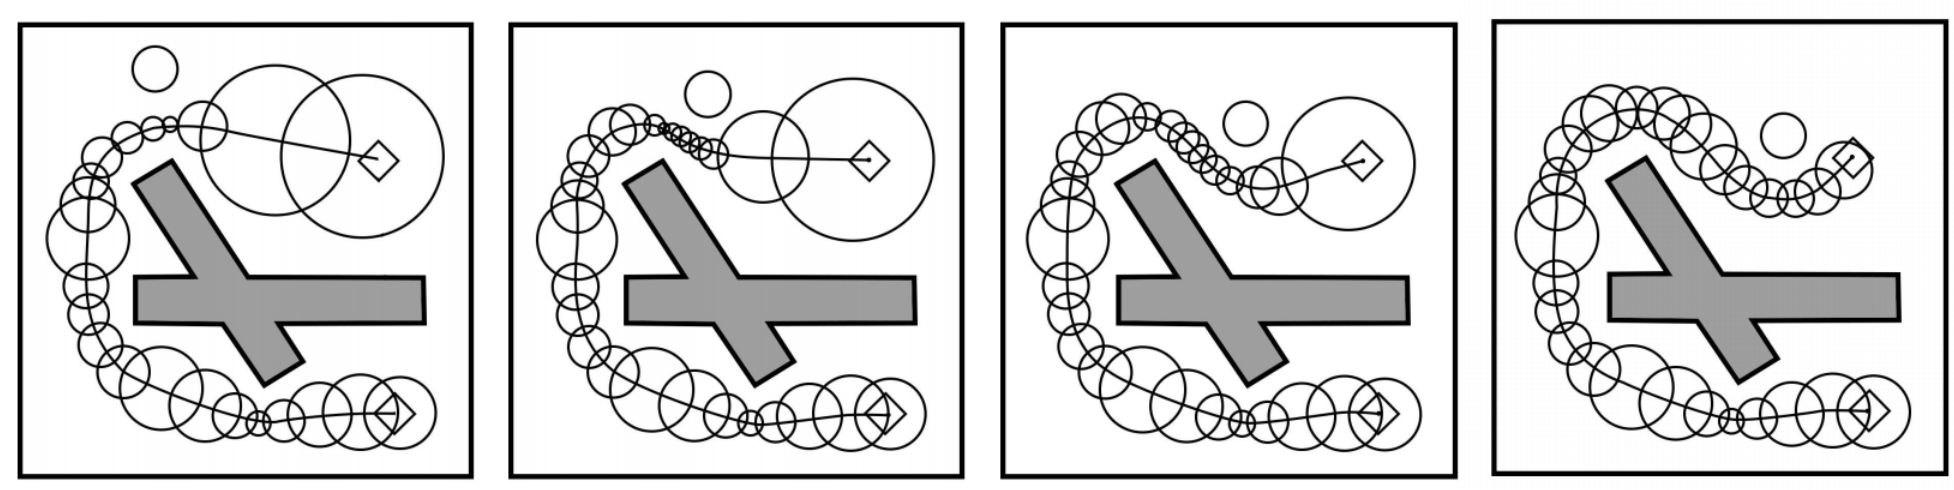
\includegraphics[width=0.7\textwidth]{images/bubbles.png}
                        \caption{基于气泡的动态避障和路径平滑}
                    \end{figure}

            \item \textbf{优点}:
                \begin{itemize}
                    \item 可实现路径平滑,解决路径存在方向突变问题,便于机器人执行
                    \item 可避免避障后偏离原路径而失去到达目标点的全局信息
                \end{itemize}
            \item \textbf{缺点}:
                \begin{itemize}
                    \item 如果环境中的变化很大,弹性带即使存在,也\textbf{可能无法变形为无碰撞路径}
                    \item 本质上还是几何空间内的路径规划,是对路径规划和避障规划的融合,\textbf{并没有考虑机器人执行时的任何运动学约束}
                \end{itemize}                
        \end{itemize}
    \item \textbf{TED(TIMED ELASTIC BAND)}
                    \begin{figure}[H]
                        \centering
                        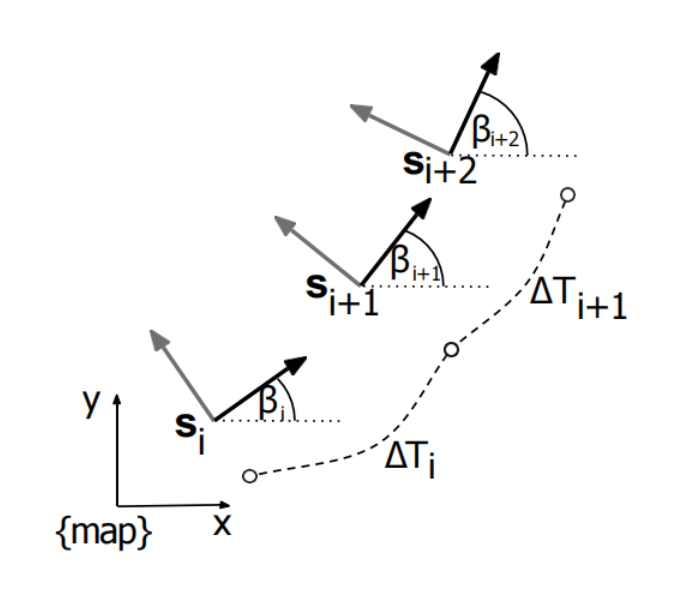
\includegraphics[width=0.35\textwidth]{images/TEB.png}
                        \caption{TEB示意图}
                    \end{figure}
        \begin{itemize}
            \item \textbf{针对问题}:
                \begin{itemize}
                    \item 增加\textbf{时间信息},将路径转化为\textbf{轨迹};
                    \item 综合考虑机器人\textbf{运动学和动力学约束},通过\textbf{加权多目标优化}对轨迹进行变形
                \end{itemize}
            \item \textbf{关键思想}:在路径的相邻位姿之间增加时间间隔
            \item \textbf{实现方法}:
                \begin{enumerate}
                    \item 在初始路径上增加默认的\textbf{关于动力学和运动学约束}的\textbf{时间信息},将初始路径转化为\textbf{初始轨迹}
                    \item 在每次迭代中,动态地\textbf{增加新的位形}或\textbf{删除已有路径位姿节点},以便修正空间和时间分辨率,与当前轨迹长度匹配
                    \item 建立\textbf{约束描述},构建超图模型,进行最优化问题求解
                    \item 验证最优化得到的轨迹是否可行:
                        \begin{itemize}
                            \item 如果可行,计算速度控制变量$v$和$\omega$,驱动机器人执行;
                            \item 如果不可行,重新初始化,检查新的和改变的路径点,判断路径点密度是否能够确保视觉或者激光扫描传感器检测到,然后转步骤2迭代
                        \end{itemize}
                \end{enumerate}
            \item \textbf{优点}:
                \begin{itemize}
                    \item 引入时间信息和动力学运动学等约束条件,将避障规划和轨迹规划有效融合
                    \item 具有较好的鲁棒性和扩展特性,可以方便的引入新的目标和约束
                \end{itemize}
            \item \textbf{缺点}:
                \begin{itemize}
                    \item 当问题规模较大、目标或者约束存在 一定冲突时,问题求解计算成本较高,会难以满足实时性要求
                \end{itemize}
            \item \textbf{具体算法}:
                \small\kaishu{
\begin{enumerate}
  \item \textbf{变量与轨迹表示}\,:\\
  路径位姿序列 $Q=\{\,\mathbf{x}_i\,\}_{i=0,\dots,n}$,其中 $\mathbf{x}_i=(x_i,y_i,\theta_i)$;时间间隔序列
  $\tau=\{\,\Delta T_i\,\}_{i=0,\dots,n-1}$。\\
  将两者合在一起的\emph{弹性带}为
  \[
    B=(Q,\tau).
  \]

  \item \textbf{问题}\,: 同时对轨迹的位姿与相邻位姿间的时间间隔进行调整与优化,实现加权多目标最优化。

  \item \textbf{最优解}\,:  
  \[
     B^{\star}=\arg\min_{B}\,f(B).
  \]

  \item \textbf{总体目标函数(加权求和)}\,:  
  \[
     f(B)=\sum\nolimits_{k}\,N\,\gamma_k\,f_k(B),
  \]
  其中 $\gamma_k$ 为权重,$N$ 为尺度/归一化因子,$f_k(\cdot)$ 为各个目标或约束对应的代价。

  \item \textbf{各项目标/约束建模}\,:  
  \begin{itemize}
    \item \emph{(1) 时间最短目标}  
    \[
       f_{\text{time}}(B)=\Big(\sum_{i=1}^{n} \mathcal{N}\,\Delta T_i\Big)^2 .
    \]
    \item \emph{(2) 约束转化为惩罚目标}\,: 对一般不等式约束 $x\le x_r$,采用多项式惩罚
    \[
      e_{\Gamma}(x,x_r,\varepsilon,S,n)\; \triangleq\;
      \begin{cases}
        \displaystyle T\!\left(\frac{x-(x_r-\varepsilon)}{S}\right)^{\!n}, & \text{if } x>x_r-\varepsilon,\\[6pt]
        0, & \text{otherwise},
      \end{cases}
    \]
    其中 $S$ 为比例缩放,$n$ 为多项式阶数,$\varepsilon$ 为小的近似偏移($S,n,\varepsilon$ 共同影响近似精度)。
    \begin{enumerate}
    \item \emph{速度与加速度约束}
    \[
      f_v=\sum_i e_{\Gamma}(v_i,v_{\max},\varepsilon,S,n),\qquad
      f_\omega=\sum_i e_{\Gamma}(\omega_i,\omega_{\max},\varepsilon,S,n),
    \]
    其中
    \[
      v_i \approx \frac{1}{\Delta T_i}\Big\|\begin{pmatrix}x_{i+1}-x_i\\ y_{i+1}-y_i\end{pmatrix}\Big\|,\qquad
      \omega_i \approx \frac{\theta_{i+1}-\theta_i}{\Delta T_i}.
    \]
    线加速度与角加速度同理,线加速度可写成
    \[
      f_a=\sum_i e_{\Gamma}(a_i,a_{\max},\varepsilon,S,n),\qquad
      a_i=\frac{2\,(v_{i+1}-v_i)}{\Delta T_i+\Delta T_{i+1}}.
    \]

    \item \emph{路径带与避障安全约束}\,: 设与路径点/障碍物 $z_j$ 的最小距离为 $d_{\min,j}$,
    \[
      f_{\text{path}}=\sum_j e_{\Gamma}\!\big(d_{\min,j},\,r_{p_{\max}},\,\varepsilon,S,n_b\big),\qquad
      f_{\text{ob}}=\sum_j e_{\Gamma}\!\big(-d_{\min,j},\,-r_{o_{\min}},\,\varepsilon,S,n_b\big),
    \]
    其中 $r_{p_{\max}}$ 为弹性带允许的最大“松弛”半径,$r_{o_{\min}}$ 为最小安全距离阈值,$n_b$ 为带宽/邻域相关参数。

    \item \emph{非完整运动学约束(差动/汽车类)}\,: 令
    \[
      \mathbf{d}_{i,i+1}=\begin{pmatrix}x_{i+1}-x_i\\[2pt]y_{i+1}-y_i\\[2pt]0\end{pmatrix},\quad
      \mathbf{h}(\theta)=\begin{pmatrix}\cos\theta\\ \sin\theta\\ 0\end{pmatrix},
    \]
    则等价目标为
    \[
      f_{\text{nh}}(\mathbf{x}_i,\mathbf{x}_{i+1})
      =\big\|\,\big(\mathbf{h}(\theta_i)+\mathbf{h}(\theta_{i+1})\big)\times \mathbf{d}_{i,i+1}\big\|^2,
    \]
    使车辆切向于段 $\mathbf{d}_{i,i+1}$(即 $\beta_i=\beta_{i+1}$ 的等价形式)。
    \begin{figure}[H]
    \centering
    \begin{minipage}[t]{0.35\textwidth}
        \centering
        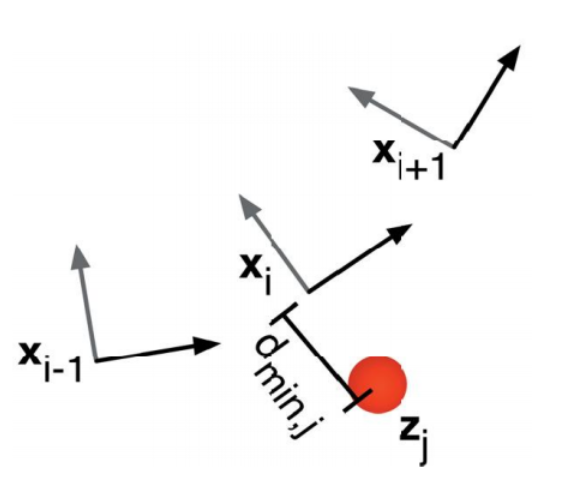
\includegraphics[width=\textwidth]{images/yueshu2.png}
        \caption{路径带与避障安全约束}
    \end{minipage}
    \begin{minipage}[t]{0.35\textwidth}
        \centering
        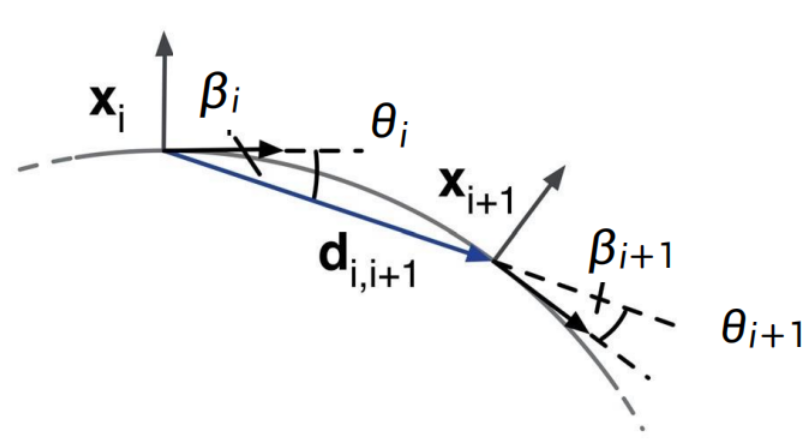
\includegraphics[width=\textwidth]{images/yueshu3.png}
        \caption{非完整运动学约束}
    \end{minipage}
\end{figure}
\end{enumerate}
  \end{itemize}

  \item \textbf{求解与实现}\,:\\
  将 $\{\mathbf{x}_i\}$ 与 $\{\Delta T_i\}$ 作为图(超图\footnote{由节点和边组成,其中一条边所能连接的节点数量不受限制,可以连接两个以上的节点})中的顶点,各项 $f_k$ 作为边/超边代价。由于大多数代价仅与局部相邻节点与时间间隔相关,问题具有\emph{稀疏性},可用图优化框架(如 \texttt{g2o}\footnote{常用的大规模稀疏非线性最小二乘求解器。})迭代求解,迭代过程中还可根据轨迹长度\emph{动态插入/删除}位姿节点以匹配时空分辨率。
\end{enumerate}
}
        \end{itemize}
\end{enumerate}
\end{document}